In this section, we present our study results by answering our research questions. For each question, we discuss the motivation behind it, the approach to answering it and finally the results obtained. 
\\

\noindent\textbf{RQ1:} \textbf{How much do logs change over time and why do the changes occur?}
\\

\noindent\textbf{Motivation}

Research has shown that logs evolve along with the code~\cite{IanContextinformation}. When logs are changed, the log  processing tools which are dependent on them also have to get updated. This results in costly maintenance effort. To understand the cost, we have to understand how frequent changes to logs are. Hence, we explore the frequency of changes to logs in our studied systems and why they are changed.\\

\noindent \textbf{Approach}

To find the frequency of log changes, we conduct a quantitative analysis on our studied systems. We use the tracked log data for each studied system as explained in Section~\ref{Methodology}. From each project, we select a random sample with 95\% confidence interval. We follow the same iterative process as in prior research~\cite{IanIcesm} to find how frequently logs change in our studied systems. \\

When logs are changed, they can be changed for several reasons. To understand the different types of log changes we perform a manual analysis on the changed logs. We select a random sample from each project such that the sample achieves 95\% confidence interval. After identifying the different types of log changes we automate the process of identification using our scripts. Figure~\ref{fig:Flowchart2} highlights the process of categorizing the log changes. For example, 
consider the logs shown below. 

\hypobox {+ LOG.info(``starting HBase HsHA Thrift server on " + Integer.toString(listenPort)); }

\hypobox {- LOG.info(``starting HBase " + implType.simpleClassName() +`` server on " + Integer.toString(listenPort)); }

We see that there can be only four possible ways in which developers change logs namely:
\begin{enumerate}
	
	\item { \textbf{Log relocation:} } The log is kept intact but moved to a different location in the file because of context changes (code around the log is changed).
	
	\item \textbf{Text change:} The text (i.e., static content) of log is changed. 
	
	\item\textbf{Variable change:} One or more variables in the log are changed (added, deleted or modified).
	
	\item \textbf{Change of log level:} The verbosity level of a log is changed.
	
	\item  \textbf{Text and variable change:} Both text and variables in the logs are changed. This is generally done when developers provide more context information, i.e, text and add/modify the relevant variables in a log.
	
\end{enumerate}

To automate the process of categorizing log changes into these categories, we first remove the logging method (i.e, LOG) and the log level (i.e, info) from the logs. We then compute the \textsl{Levenshtein ratio} between each term within the parentheses. In the above case we find that `+ Integer.toString(listenPort)' has \textsl{Levenshtein ratio} of 1, implying they are identical and the \textsl{Levenshtein ratio} between `starting HBase HsHA Thrift server on' and `starting HBase' is 0.56. This suggests there is some similarity between the two strings and the variable is constant which implies its a text change. 

After identifying the different types of log changes in the studied systems, we find the number of the developers responsible for the log changes and also if they own the file which contains the log. We use the committer name available from the `git log' to sum the number of developers who change a log. To find if a developer owns a file we calculate the ratio of number of lines written by him to the total lines of code using the `blame' command available in git. 

% ownership of file using the `blame' command available in git i.e.., if two developers are responsible for a file, but one has written 100 of the 150 lines of code, we calculate his 
%\begin{enumerate}
%	
%	\item { \textbf{Log relocation:} } The log is kept intact but moved to a different location in the file because of context changes (code around the log is changed).
%	
%	\item \textbf{Text change:} The text (i.e., static content) of log is changed. 
%	
%	\item\textbf{Variable change:} One or more variables in the log are changed (added, deleted or modified).
%	
%	\item \textbf{Change of log level:} The verbosity level of a log is changed.
%	
%	\item  \textbf{Text and variable change:} Both text and variables in the logs are changed. This is generally done when developers provide more context information, i.e, text and add/modify the relevant variables in a log.
%	
%\end{enumerate}
% 
\begin{figure}[tb]
	\centering
	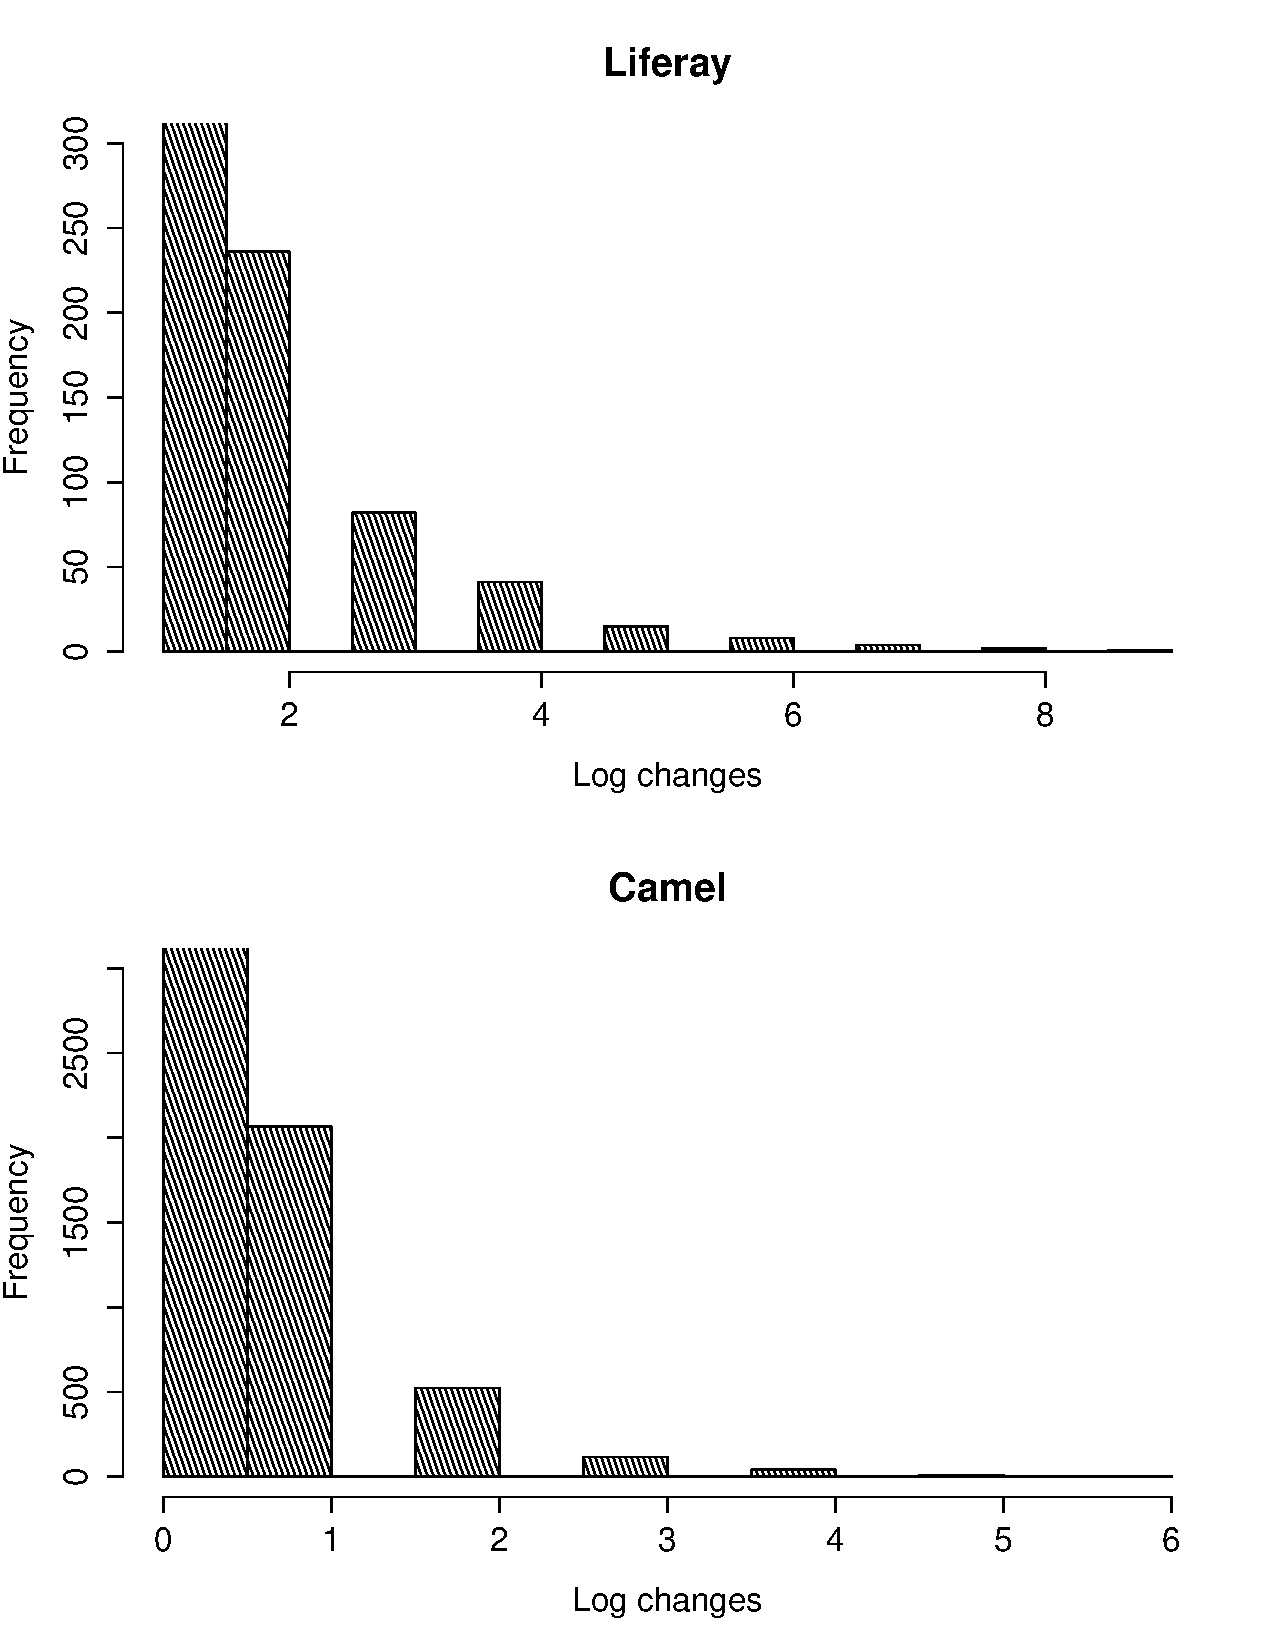
\includegraphics[width=0.7\linewidth]{RQ1_Liferay_Camel_Logchangefreq}
	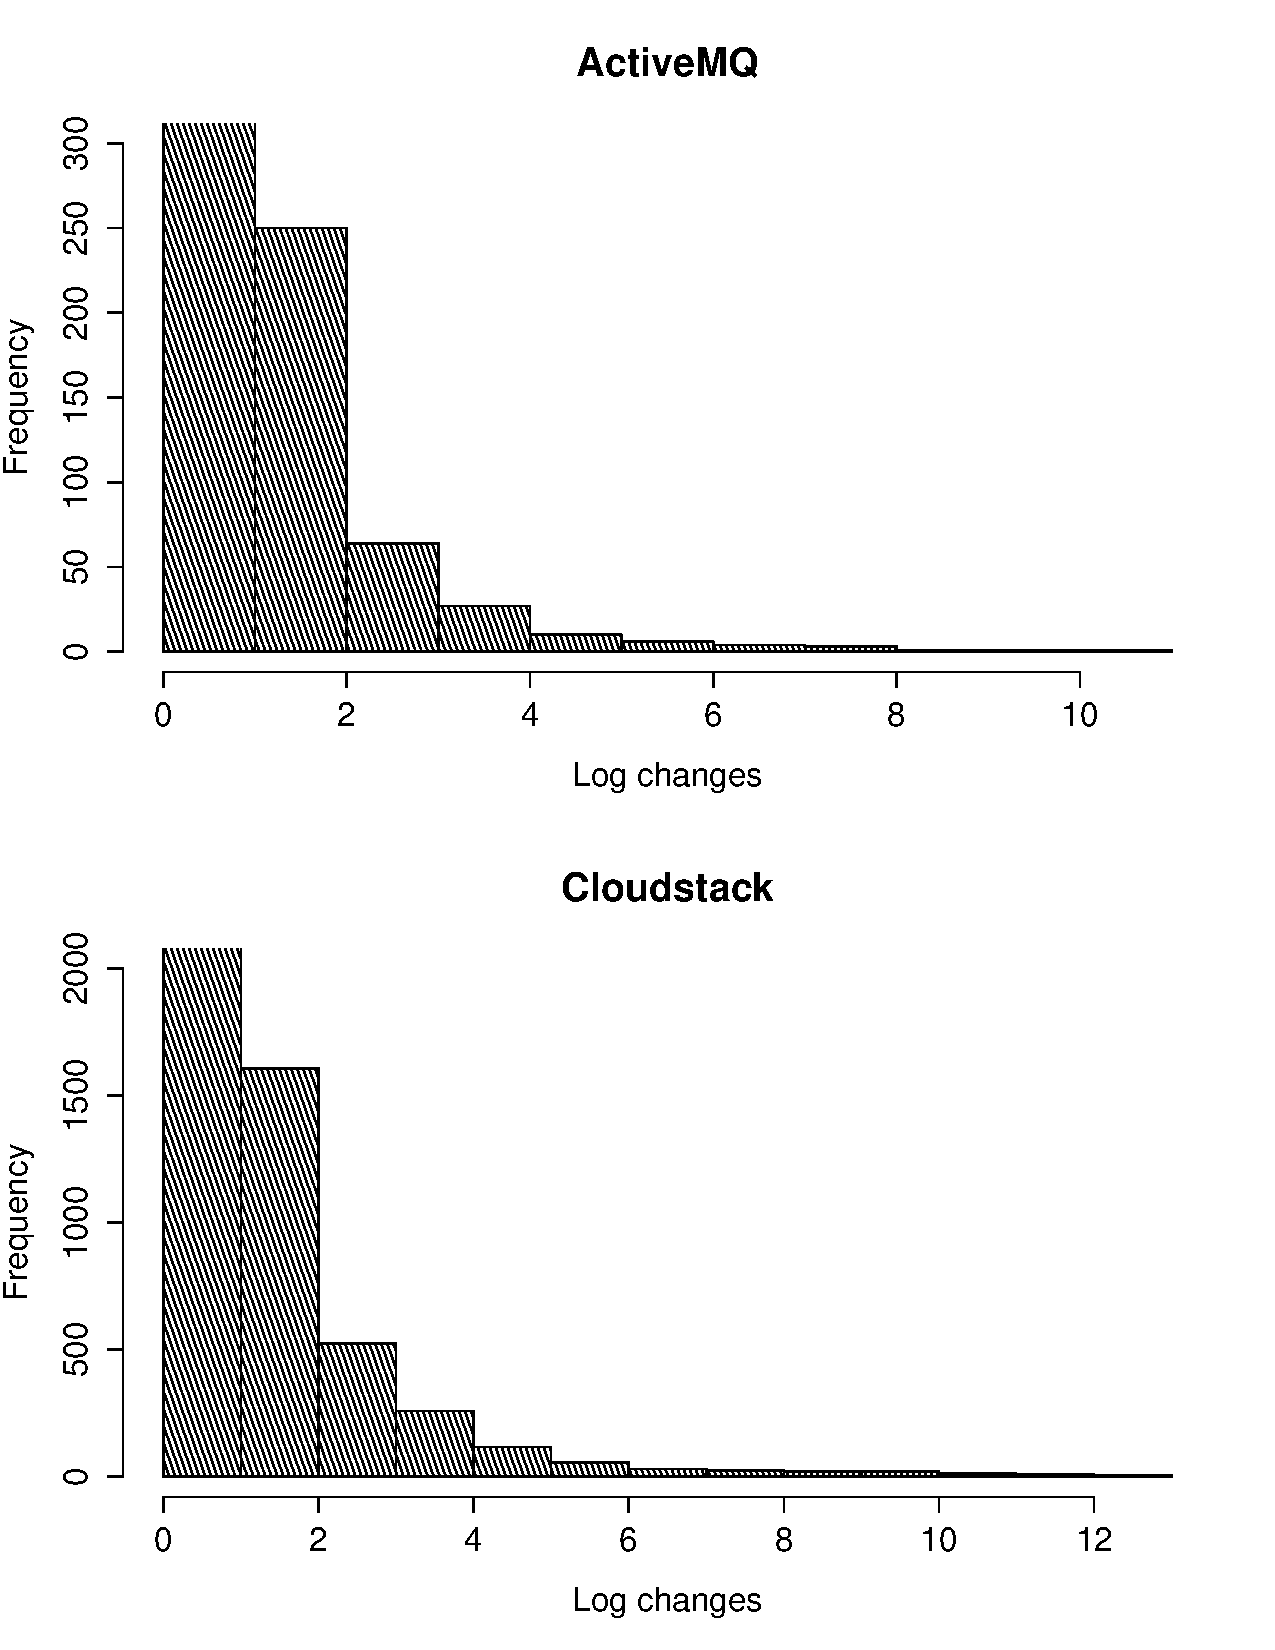
\includegraphics[width=0.7\linewidth]{RQ1_Cloud_Active_Logchangefreq}
	\caption{Frequency of log changes in the studied systems.}
	\label{fig:RQ1_Liferay_Camel_Logchangefreq}
\end{figure}
\begin{figure}[tb]
	\centering
	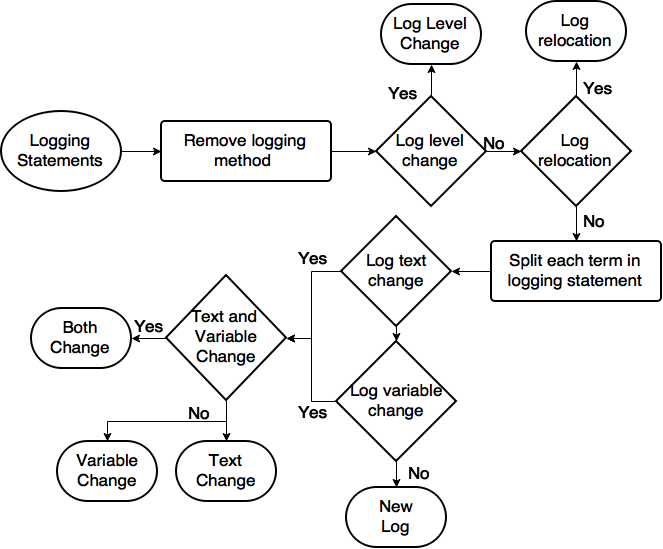
\includegraphics[width=0.75\linewidth]{Flowchart2}
	\caption{Flowchart to categorize the different types of log changes that occur}
	\label{fig:Flowchart2}
\end{figure}



\noindent \textbf{Results}

\textbf{We find that developers change 20-80\% of the logs across our studied systems as shown in Figure~\ref{fig:RQ1_Liferay_Camel_Logchangefreq}}. Based on frequency of changes, we categorize logs into 3 categories namely: a) Frequently Changed, b) Changed and c) Never Changed as shown in Table~\ref{tba:logchangeDistribution}. If a log is changed more than three times it is categorized as `Frequently Changed'. If it is changed fewer 1 to 3 times it is categorized under `changed' and if there is no changes made it is categorized under `Never Changed'. We see that a majority of logs never change in HBase and Life Ray and the logs in ActiveMQ and CloudStack are changed at-least once. This may be because Camel and Liferay have fewer logs per source code (i.e., lower log density) when compared to ActiveMQ and CloudStack as seen in Table~\ref{tba:overviewsystems}. 
%{\suhas{ I have question Can i tell here that in RQ2 we find log density to be imporatnt factor in stability of logs ?? }}

% are application layer software which  rely less on logs as they are middle-ware/application software, whereas ActiveMQ and CloudStack are service software.


\begin{table*}
	\centering
	\caption{Distribution of log changes in different projects}
	\label{tba:logchangeDistribution}
	\begin{tabular}{l|>{\centering}p{.1\columnwidth}>{\centering}p{.01\columnwidth} 
			p{0.01\columnwidth} }
	\cline{1-4}  	\multicolumn{1}{|c}{Projects}    & \multicolumn{1}{|c}{Never Changed (\%) }  &  \multicolumn{1}{|c}{Changed (\%) }	   &  \multicolumn{1}{|c}{Frequently Changed (\%) }\\ \cline{1-4}   

		Life Ray      & 78.67     & 19.66 & 1.66           \\
		
		Camel      & 55.43    & 37.32 & 7.25            \\
		ActiveMq   & 34.78     & 62.02 & 3.20           \\
		CloudStack & 19.68     & 68.61 & 11.71          \\ \cline{1-4}
	\end{tabular}
\end{table*}

\begin{figure}[tb]

\centering
  \subfloat{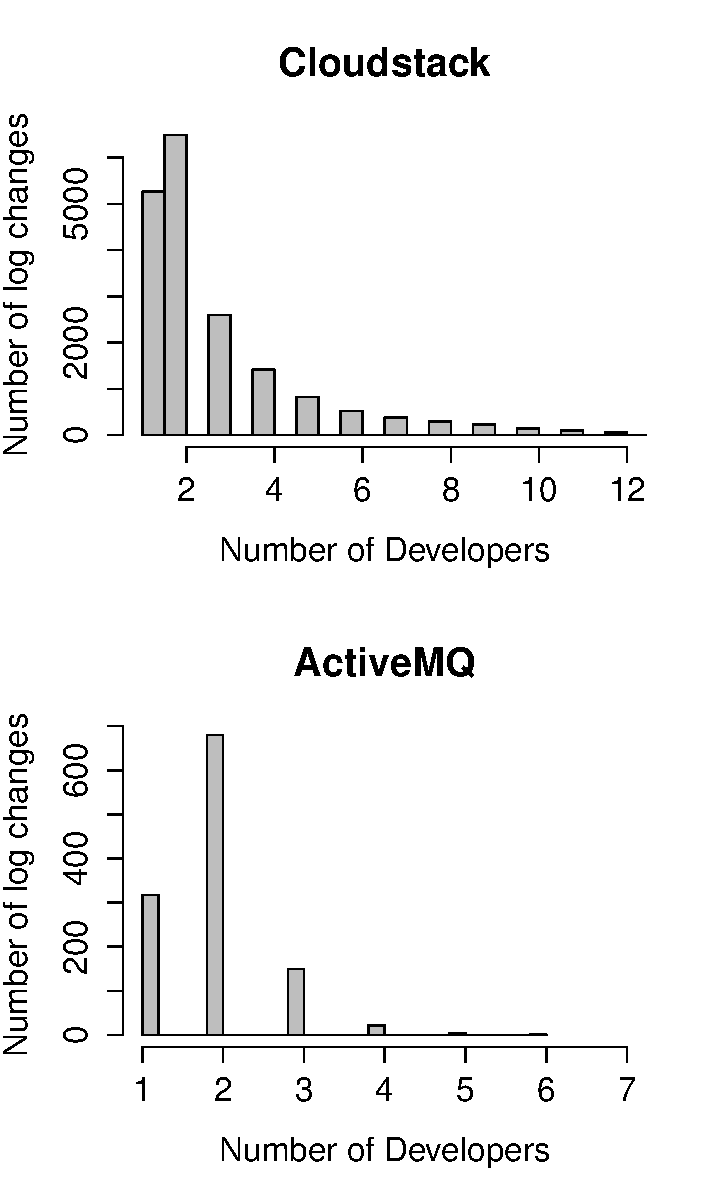
\includegraphics[width=0.5\linewidth]{CA_numberofDevelopers}\label{fig:f1}}
  \hfill
  \subfloat{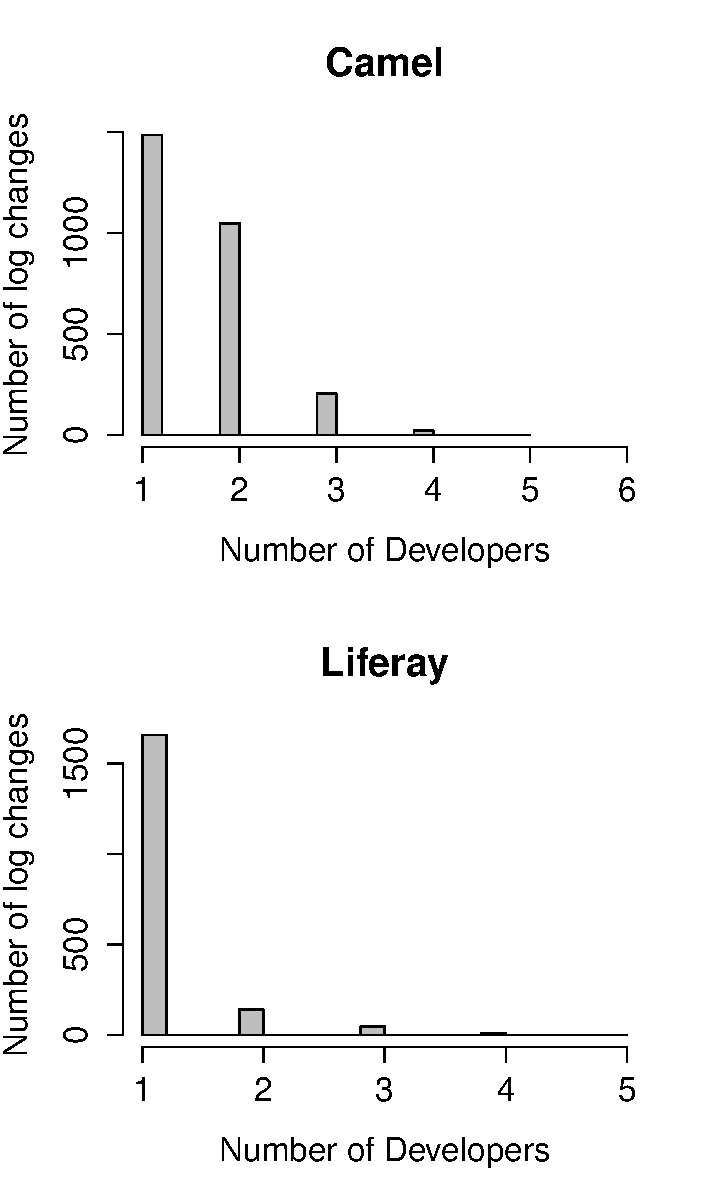
\includegraphics[width=0.5\linewidth]{CL_numberofDevelopers}\label{fig:f2}}
\caption{Number of developers responsible for changing logs}
\label{fig:NumberofDevelopers}
\end{figure}
We find that relocation occurs more often than other types of log changes. We find that in all the studied systems log relocation occurs more than 49\%. As log relocations have no changes to the text or variables in logs, their impact on log processing tools is limited. Hence we exclude log relocation changes from our datasets. 


%From manually analyzing the changed logs, we identify five types of log changes (i.e., changes to verbosity levels, log context, logged variables, both context and variable and relocation of log).  Table~\ref{tba:logtype} shows their distributions. When there is overlapping of the different types of log changes, we categorize them as newly added log and track changes made to it.
We find that logs are changed mainly by developers who introduce the log within our studied systems. From Figure~\ref{fig:NumberofDevelopers} we see that in three of the studied systems, a single developer is responsible for majority of the log changes. 
\begin{figure}[tb]
\centering
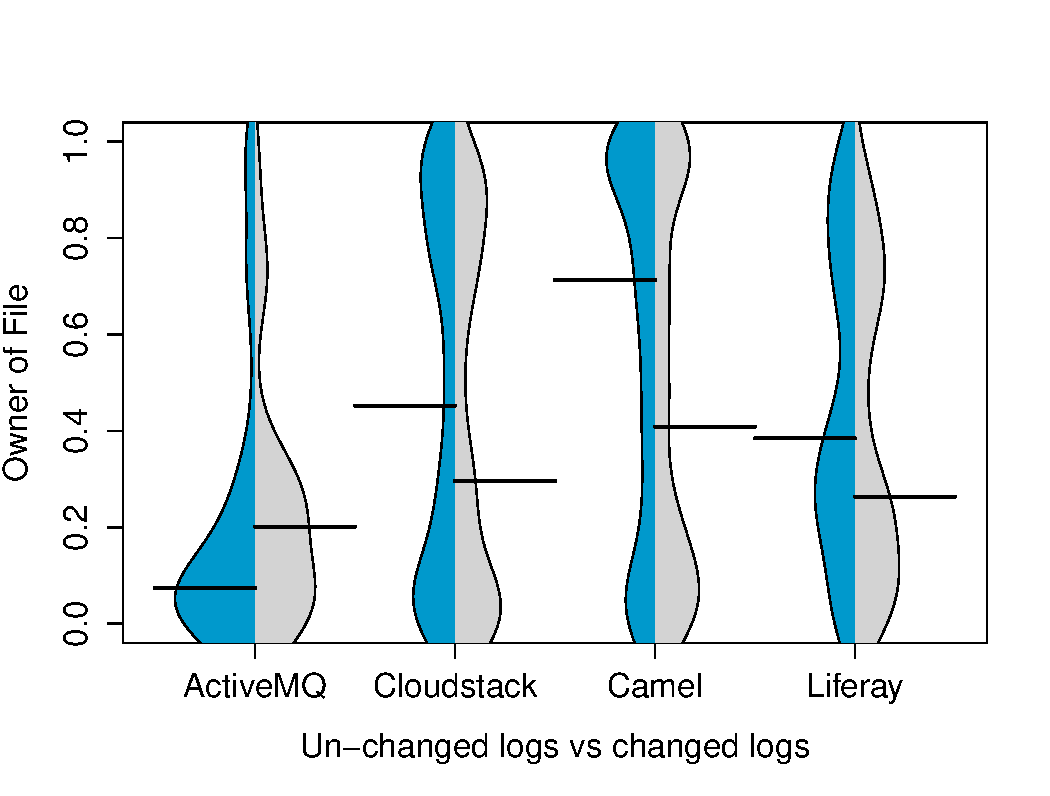
\includegraphics[width=1\linewidth]{ChangedvsUnchangedlogs}
\caption{Distribution of file ownership against log change in the studied systems}
\label{fig:ChangedvsUnchangedlogs}
\end{figure}


\begin{table*}[t]
	\centering
	\caption{Distribution of log changes in different projects}
	\label{tba:logtype}
	\begin{tabular}{l|llll}
		\cline{1-5}  	\multicolumn{1}{|c}{Projects}    & \multicolumn{1}{|c}{ Life Ray }  &  \multicolumn{1}{|c}{ Cloud Stack}	   &  \multicolumn{1}{|c}{ Active-MQ }  & 
		 \multicolumn{1}{|c|}{ Camel } \\ \cline{1-5}   
		
		Log relocation (\%)       & 73.5     & 78.85 &  63.27  & 49.72         \\
		
		Log text change (\%)      & 20.11    & 6.37 & 5.97    & 7.59       \\
		Log variable change (\%)   & 3.10     & 7.21 & 6.91 &  8.29     \\
		Change of log level (\%) & 0.87   & 1.15 & 1.76  &  3.79       \\ 
		Text and variable change (\%) & 2.33     & 6.39 & 22.0   &  30.59    \\ \cline{1-5}
	\end{tabular}
\end{table*}

\textbf{We see that logs are changed by developers who have little ownership over the file.} From Figure~\ref{fig:ChangedvsUnchangedlogs} we see that in three of the studied systems logs are changed by developers who have lesser ownership on files than the developers who introduce the log. This suggests that logs do not have strong ownership characteristics and can be changed by developers than one introducing the logs.

\hypobox { 45\% of the logs are changed atleast once in three of our studied systems. We find that over 49\% of these log changes are due to log relocation. The changes are made to the text (i.e., static content), variable and log level. This suggests that developers change logs extensively throughout the lifecyle of a software and developers might dedicate significant amount of time to update and maintain logs}
%	We find that about 3-11 \% of logs are changed frequently. This suggests that log processing tools which run on these systems need constant maintenance from developers

